%
% 6.S077 problem set solutions template
%
\documentclass[12pt,twoside]{article}
\usepackage{bbm}

\newcommand{\name}{}

\usepackage{amssymb}
\usepackage{amsmath}
\usepackage{graphicx}
\usepackage{latexsym}
\usepackage{times,url}
\usepackage{cprotect}
\usepackage{listings}
\usepackage{graphicx}
\usepackage[table]{xcolor}
\usepackage[letterpaper]{geometry}
\usepackage{tikz-qtree}
\usepackage{enumerate}

\newcommand{\profs}{Mauricio Karchmer, Aleksander Madry, Bruce Tidor}
\newcommand{\subj}{6.046}
\newcommand{\ttt}[1]{{\tt\small #1}}

\definecolor{dkgreen}{rgb}{0,0.6,0}
\definecolor{gray}{rgb}{0.5,0.5,0.5}
\definecolor{mauve}{rgb}{0.58,0,0.82}

\lstset{
  language=Python,
  aboveskip=1pc,
  belowskip=1pc,
  basicstyle={\footnotesize\ttfamily},
  numbers=left,
  showstringspaces=false,
  numberstyle=\tiny\color{gray},
  keywordstyle=\color{blue},
  commentstyle=\color{dkgreen},
  stringstyle=\color{mauve},
}

\tikzset{
  % every node/.style={minimum width=2em,draw,circle},
  % level 1/.style={sibling distance=2cm},
  level distance=1cm,
  edge from parent/.style=
  {draw,edge from parent path={(\tikzparentnode) -- (\tikzchildnode)}},
}

\newif\ifHideSolutions
\newcommand{\solution}[1]{\color{dkgreen}\textbf{Solution: }#1\color{black}}
\newcommand{\rubric}[1]{\color{dkgreen}{\bf Rubric:} #1\color{black}}

% \HideSolutionsfalse
% \ifHideSolutions
%   \renewcommand{\solution}[1]{}
%   \renewcommand{\rubric}[1]{}
% \fi

\newlength{\toppush}
\setlength{\toppush}{2\headheight}
\addtolength{\toppush}{\headsep}

\newcommand{\htitle}[2]{\noindent\vspace*{-\toppush}\newline\parbox{6.5in}
{\textit{Design and Analysis of Algorithms}\hfill\name\newline
Massachusetts Institute of Technology \hfill #2\newline
\profs\hfill #1 \vspace*{-.5ex}\newline
\mbox{}\hrulefill\mbox{}}\vspace*{1ex}\mbox{}\newline
\begin{center}{\Large\bf #1}\end{center}}

\newcommand{\handout}[2]{\thispagestyle{empty}
 \markboth{#1}{#1}
 \pagestyle{myheadings}\htitle{#1}{#2}}

\newcommand{\lecture}[3]{\thispagestyle{empty}
 \markboth{Lecture #1: #2}{Lecture #1: #2}
 \pagestyle{myheadings}\htitle{Lecture #1: #2}{#3}}

\newcommand{\htitlewithouttitle}[2]{\noindent\vspace*{-\toppush}\newline\parbox{6.5in}
{\textit{Design and Analysis of Algorithms}\hfill#2\newline
Massachusetts Institute of Technology \hfill 6.046\newline
\profs\hfill Handout #1\vspace*{-.5ex}\newline
\mbox{}\hrulefill\mbox{}}\vspace*{1ex}\mbox{}\newline}

\newcommand{\handoutwithouttitle}[2]{\thispagestyle{empty}
 \markboth{Handout \protect\ref{#1}}{Handout \protect\ref{#1}}
 \pagestyle{myheadings}\htitlewithouttitle{\protect\ref{#1}}{#2}}

\newcommand{\exam}[2]{% parameters: exam name, date
 \thispagestyle{empty}
 \markboth{\hspace{1cm}\subj\ #1\hspace{1in}Name\hrulefill\ \ }%
          {\subj\ #1\hspace{1in}Name\hrulefill\ \ }
 \pagestyle{myheadings}\examtitle{#1}{#2}
 \renewcommand{\theproblem}{Problem \arabic{problemnum}}
}
\newcommand{\examsolutions}[3]{% parameters: handout, exam name, date
 \thispagestyle{empty}
 \markboth{Handout \protect\ref{#1}: #2}{Handout \protect\ref{#1}: #2}
% \pagestyle{myheadings}\htitle{\protect\ref{#1}}{#2}{#3}
 \pagestyle{myheadings}\examsolutionstitle{\protect\ref{#1}} {#2}{#3}
 \renewcommand{\theproblem}{Problem \arabic{problemnum}}
}
\newcommand{\examsolutionstitle}[3]{\noindent\vspace*{-\toppush}\newline\parbox{6.5in}
{\textit{Design and Analysis of Algorithms}\hfill#3\newline
Massachusetts Institute of Technology \hfill 6.046\newline
%Singapore-MIT Alliance \hfill SMA5503\newline
\profs\hfill Handout #1\vspace*{-.5ex}\newline
\mbox{}\hrulefill\mbox{}}\vspace*{1ex}\mbox{}\newline
\begin{center}{\Large\bf #2}\end{center}}

\newcommand{\takehomeexam}[2]{% parameters: exam name, date
 \thispagestyle{empty}
 \markboth{\subj\ #1\hfill}{\subj\ #1\hfill}
 \pagestyle{myheadings}\examtitle{#1}{#2}
 \renewcommand{\theproblem}{Problem \arabic{problemnum}}
}

\makeatletter
\newcommand{\exambooklet}[2]{% parameters: exam name, date
 \thispagestyle{empty}
 \markboth{\subj\ #1}{\subj\ #1}
 \pagestyle{myheadings}\examtitle{#1}{#2}
 \renewcommand{\theproblem}{Problem \arabic{problemnum}}
 \renewcommand{\problem}{\newpage
 \item \let\@currentlabel=\theproblem
 \markboth{\subj\ #1, \theproblem}{\subj\ #1, \theproblem}}
}
\makeatother


\newcommand{\examtitle}[2]{\noindent\vspace*{-\toppush}\newline\parbox{6.5in}
{\textit{Design and Analysis of Algorithms}\hfill#2\newline
Massachusetts Institute of Technology \hfill 6.046 Spring 2019\newline
%Singapore-MIT Alliance \hfill SMA5503\newline
\profs\hfill #1\vspace*{-.5ex}\newline
\mbox{}\hrulefill\mbox{}}\vspace*{1ex}\mbox{}\newline
\begin{center}{\Large\bf #1}\end{center}}

\newcommand{\grader}[1]{\hspace{1cm}\textsf{\textbf{#1}}\hspace{1cm}}

\newcommand{\points}[1]{[#1 points]\ }
\newcommand{\parts}[1]
{
  \ifnum#1=1
  (1 part)
  \else
  (#1 parts)
  \fi
  \ 
}

\newcommand{\bparts}{\begin{problemparts}}
\newcommand{\eparts}{\end{problemparts}}
\newcommand{\ppart}{\problempart}

%\newcommand{\lg} {lg\ }

\setlength{\oddsidemargin}{0pt}
\setlength{\evensidemargin}{0pt}
\setlength{\textwidth}{6.5in}
\setlength{\topmargin}{0in}
\setlength{\textheight}{8.5in}


\newcommand{\Spawn}{{\bf spawn} }
\newcommand{\Sync}{{\bf sync}}

\newcommand{\cif}[1]{\mbox{if $#1$}}
\newcommand{\cwhen}[1]{\mbox{when $#1$}}

\newcounter{problemnum}
\newcommand{\theproblem}{Problem \theproblemsetnum-\arabic{problemnum}}
\newenvironment{problems}{
        \begin{list}{{\bf \theproblem. \hspace*{0.5em}}}
        {\setlength{\leftmargin}{0em}
         \setlength{\rightmargin}{0em}
         \setlength{\labelwidth}{0em}
         \setlength{\labelsep}{0em}
         \usecounter{problemnum}}}{\end{list}}
\makeatletter
\newcommand{\problem}[1][{}]{\item \let\@currentlabel=\theproblem \textbf{#1}}
\makeatother

\newcounter{problempartnum}[problemnum]
\newenvironment{problemparts}{
        \begin{list}{{\bf (\alph{problempartnum})}}
        {\setlength{\leftmargin}{2.5em}
         \setlength{\rightmargin}{2.5em}
         \setlength{\labelsep}{0.5em}}}{\end{list}}
\newcommand{\problempart}{\addtocounter{problempartnum}{1}\item}

\newenvironment{truefalseproblemparts}{
        \begin{list}{{\bf (\alph{problempartnum})\ \ \ T\ \ F\hfil}}
        {\setlength{\leftmargin}{4.5em}
         \setlength{\rightmargin}{2.5em}
         \setlength{\labelsep}{0.5em}
         \setlength{\labelwidth}{4.5em}}}{\end{list}}

\newcounter{exercisenum}
\newcommand{\theexercise}{Exercise \theproblemsetnum-\arabic{exercisenum}}
\newenvironment{exercises}{
        \begin{list}{{\bf \theexercise. \hspace*{0.5em}}}
        {\setlength{\leftmargin}{0em}
         \setlength{\rightmargin}{0em}
         \setlength{\labelwidth}{0em}
         \setlength{\labelsep}{0em}
        \usecounter{exercisenum}}}{\end{list}}
\makeatletter
\newcommand{\exercise}{\item \let\@currentlabel=\theexercise}
\makeatother

\newcounter{exercisepartnum}[exercisenum]
%\newcommand{\problem}[1]{\medskip\mbox{}\newline\noindent{\bf Problem #1.}\hspace*{1em}}
%\newcommand{\exercise}[1]{\medskip\mbox{}\newline\noindent{\bf Exercise #1.}\hspace*{1em}}

\newenvironment{exerciseparts}{
        \begin{list}{{\bf (\alph{exercisepartnum})}}
        {\setlength{\leftmargin}{2.5em}
         \setlength{\rightmargin}{2.5em}
         \setlength{\labelsep}{0.5em}}}{\end{list}}
\newcommand{\exercisepart}{\addtocounter{exercisepartnum}{1}\item}


% Macros to make captions print with small type and 'Figure xx' in bold.
\makeatletter
\def\fnum@figure{{\bf Figure \thefigure}}
\def\fnum@table{{\bf Table \thetable}}
\let\@mycaption\caption
%\long\def\@mycaption#1[#2]#3{\addcontentsline{\csname
%  ext@#1\endcsname}{#1}{\protect\numberline{\csname 
%  the#1\endcsname}{\ignorespaces #2}}\par
%  \begingroup
%    \@parboxrestore
%    \small
%    \@makecaption{\csname fnum@#1\endcsname}{\ignorespaces #3}\par
%  \endgroup}
%\def\mycaption{\refstepcounter\@captype \@dblarg{\@mycaption\@captype}}
%\makeatother
\let\mycaption\caption
%\newcommand{\figcaption}[1]{\mycaption[]{#1}}

\newcounter{totalcaptions}
\newcounter{totalart}

\newcommand{\figcaption}[1]{\addtocounter{totalcaptions}{1}\caption[]{#1}}

% \psfigures determines what to do for figures:
%       0 means just leave vertical space
%       1 means put a vertical rule and the figure name
%       2 means insert the PostScript version of the figure
%       3 means put the figure name flush left or right
\newcommand{\psfigures}{0}
\newcommand{\spacefigures}{\renewcommand{\psfigures}{0}}
\newcommand{\rulefigures}{\renewcommand{\psfigures}{1}}
\newcommand{\macfigures}{\renewcommand{\psfigures}{2}}
\newcommand{\namefigures}{\renewcommand{\psfigures}{3}}

\newcommand{\figpart}[1]{{\bf (#1)}\nolinebreak[2]\relax}
\newcommand{\figparts}[2]{{\bf (#1)--(#2)}\nolinebreak[2]\relax}


\macfigures     % STATE

% When calling \figspace, make sure to leave a blank line afterward!!
% \widefigspace is for figures that are more than 28pc wide.
\newlength{\halffigspace} \newlength{\wholefigspace}
\newlength{\figruleheight} \newlength{\figgap}
\newcommand{\setfiglengths}{\ifnum\psfigures=1\setlength{\figruleheight}{\hruleheight}\setlength{\figgap}{1em}\else\setlength{\figruleheight}{0pt}\setlength{\figgap}{0em}\fi}
\newcommand{\figspace}[2]{\ifnum\psfigures=0\leavefigspace{#1}\else%
\setfiglengths%
\setlength{\wholefigspace}{#1}\setlength{\halffigspace}{.5\wholefigspace}%
\rule[-\halffigspace]{\figruleheight}{\wholefigspace}\hspace{\figgap}#2\fi}
\newlength{\widefigspacewidth}
% Make \widefigspace put the figure flush right on the text page.
\newcommand{\widefigspace}[2]{
\ifnum\psfigures=0\leavefigspace{#1}\else%
\setfiglengths%
\setlength{\widefigspacewidth}{28pc}%
\addtolength{\widefigspacewidth}{-\figruleheight}%
\setlength{\wholefigspace}{#1}\setlength{\halffigspace}{.5\wholefigspace}%
\makebox[\widefigspacewidth][r]{#2\hspace{\figgap}}\rule[-\halffigspace]{\figruleheight}{\wholefigspace}\fi}
\newcommand{\leavefigspace}[1]{\setlength{\wholefigspace}{#1}\setlength{\halffigspace}{.5\wholefigspace}\rule[-\halffigspace]{0em}{\wholefigspace}}

% Commands for including figures with macpsfig.
% To use these commands, documentstyle ``macpsfig'' must be specified.
\newlength{\macfigfill}
\makeatother
\newlength{\bbx}
\newlength{\bby}
\newcommand{\macfigure}[5]{\addtocounter{totalart}{1}
\ifnum\psfigures=2%
\setlength{\bbx}{#2}\addtolength{\bbx}{#4}%
\setlength{\bby}{#3}\addtolength{\bby}{#5}%
\begin{flushleft}
\ifdim#4>28pc\setlength{\macfigfill}{#4}\addtolength{\macfigfill}{-28pc}\hspace*{-\macfigfill}\fi%
\mbox{\psfig{figure=./#1.ps,%
bbllx=#2,bblly=#3,bburx=\bbx,bbury=\bby}}
\end{flushleft}%
\else\ifdim#4>28pc\widefigspace{#5}{#1}\else\figspace{#5}{#1}\fi\fi}
\makeatletter

\newlength{\savearraycolsep}
\newcommand{\narrowarray}[1]{\setlength{\savearraycolsep}{\arraycolsep}\setlength{\arraycolsep}{#1\arraycolsep}}
\newcommand{\normalarray}{\setlength{\arraycolsep}{\savearraycolsep}}

\newcommand{\hint}{{\em Hint:\ }}

% Macros from /th/u/clr/mac.tex

\newcommand{\set}[1]{\left\{ #1 \right\}}
\newcommand{\abs}[1]{\left| #1\right|}
\newcommand{\card}[1]{\left| #1\right|}
\newcommand{\floor}[1]{\left\lfloor #1 \right\rfloor}
\newcommand{\ceil}[1]{\left\lceil #1 \right\rceil}
\newcommand{\ang}[1]{\ifmmode{\left\langle #1 \right\rangle}
   \else{$\left\langle${#1}$\right\rangle$}\fi}
        % the \if allows use outside mathmode,
        % but will swallow following space there!
\newcommand{\paren}[1]{\left( #1 \right)}
\newcommand{\bracket}[1]{\left[ #1 \right]}
\newcommand{\prob}[1]{\Pr\left\{ #1 \right\}}
\newcommand{\Var}{\mathop{\rm Var}\nolimits}
\newcommand{\expect}[1]{{\rm E}\left[ #1 \right]}
\newcommand{\expectsq}[1]{{\rm E}^2\left[ #1 \right]}
\newcommand{\variance}[1]{{\rm Var}\left[ #1 \right]}
\renewcommand{\choose}[2]{{{#1}\atopwithdelims(){#2}}}
\def\pmod#1{\allowbreak\mkern12mu({\rm mod}\,\,#1)}
\newcommand{\matx}[2]{\left(\begin{array}{*{#1}{c}}#2\end{array}\right)}
\newcommand{\Adj}{\mathop{\rm Adj}\nolimits}

\newtheorem{theorem}{Theorem}
\newtheorem{lemma}[theorem]{Lemma}
\newtheorem{corollary}[theorem]{Corollary}
\newtheorem{xample}{Example}
\newtheorem{definition}{Definition}
\newenvironment{example}{\begin{xample}\rm}{\end{xample}}
\newcommand{\proof}{\noindent{\em Proof.}\hspace{1em}}
\def\squarebox#1{\hbox to #1{\hfill\vbox to #1{\vfill}}}
\newcommand{\qedbox}{\vbox{\hrule\hbox{\vrule\squarebox{.667em}\vrule}\hrule}}
\newcommand{\qed}{\nopagebreak\mbox{}\hfill\qedbox\smallskip}
\newcommand{\eqnref}[1]{(\protect\ref{#1})}

%%\newcommand{\twodots}{\mathinner{\ldotp\ldotp}}
\newcommand{\transpose}{^{\mbox{\scriptsize \sf T}}}
\newcommand{\amortized}[1]{\widehat{#1}}

\newcommand{\punt}[1]{}

%%% command for putting definitions into boldface
% New style for defined terms, as of 2/23/88, redefined by THC.
\newcommand{\defn}[1]{{\boldmath\textit{\textbf{#1}}}}
\newcommand{\defi}[1]{{\textit{\textbf{#1\/}}}}

\newcommand{\red}{\leq_{\rm P}}
\newcommand{\lang}[1]{%
\ifmmode\mathord{\mathcode`-="702D\rm#1\mathcode`\-="2200}\else{\rm#1}\fi}

%\newcommand{\ckt}[1]{\ifmmode\mathord{\mathcode`-="702D\sc #1\mathcode`\-="2200}\else$\mathord{\mathcode`-="702D\sc #1\mathcode`\-="2200}$\fi}
\newcommand{\ckt}[1]{\ifmmode \sc #1\else$\sc #1$\fi}

%% Margin notes - use \notesfalse to turn off notes.
\setlength{\marginparwidth}{0.6in}
\reversemarginpar
\newif\ifnotes
\notestrue
\newcommand{\longnote}[1]{
  \ifnotes
    {\medskip\noindent Note: \marginpar[\hfill$\Longrightarrow$]
      {$\Longleftarrow$}{#1}\medskip}
  \fi}
\newcommand{\note}[1]{
  \ifnotes
    {\marginpar{\tiny \raggedright{#1}}}
  \fi}


\newcommand{\reals}{\mathbbm{R}}
\newcommand{\integers}{\mathbbm{Z}}
\newcommand{\naturals}{\mathbbm{N}}
\newcommand{\rationals}{\mathbbm{Q}}
\newcommand{\complex}{\mathbbm{C}}

\newcommand{\oldreals}{{\bf R}}
\newcommand{\oldintegers}{{\bf Z}}
\newcommand{\oldnaturals}{{\bf N}}
\newcommand{\oldrationals}{{\bf Q}}
\newcommand{\oldcomplex}{{\bf C}}

\newcommand{\w}{\omega}                 %% for fft chapter

\newenvironment{closeitemize}{\begin{list}
{$\bullet$}
{\setlength{\itemsep}{-0.2\baselineskip}
\setlength{\topsep}{0.2\baselineskip}
\setlength{\parskip}{0pt}}}
{\end{list}}

% These are necessary within a {problems} environment in order to restore
% the default separation between bullets and items.
\newenvironment{normalitemize}{\setlength{\labelsep}{0.5em}\begin{itemize}}
                              {\end{itemize}}
\newenvironment{normalenumerate}{\setlength{\labelsep}{0.5em}\begin{enumerate}}
                                {\end{enumerate}}

%\def\eqref#1{Equation~(\ref{eq:#1})}
%\newcommand{\eqref}[1]{Equation (\ref{eq:#1})}
\newcommand{\eqreftwo}[2]{Equations (\ref{eq:#1}) and~(\ref{eq:#2})}
\newcommand{\ineqref}[1]{Inequality~(\ref{ineq:#1})}
\newcommand{\ineqreftwo}[2]{Inequalities (\ref{ineq:#1}) and~(\ref{ineq:#2})}

\newcommand{\figref}[1]{Figure~\ref{fig:#1}}
\newcommand{\figreftwo}[2]{Figures \ref{fig:#1} and~\ref{fig:#2}}

\newcommand{\liref}[1]{line~\ref{li:#1}}
\newcommand{\Liref}[1]{Line~\ref{li:#1}}
\newcommand{\lirefs}[2]{lines \ref{li:#1}--\ref{li:#2}}
\newcommand{\Lirefs}[2]{Lines \ref{li:#1}--\ref{li:#2}}
\newcommand{\lireftwo}[2]{lines \ref{li:#1} and~\ref{li:#2}}
\newcommand{\lirefthree}[3]{lines \ref{li:#1}, \ref{li:#2}, and~\ref{li:#3}}

\newcommand{\lemlabel}[1]{\label{lem:#1}}
\newcommand{\lemref}[1]{Lemma~\ref{lem:#1}} 

\newcommand{\exref}[1]{Exercise~\ref{ex:#1}}

\newcommand{\handref}[1]{Handout~\ref{#1}}

\newcommand{\defref}[1]{Definition~\ref{def:#1}}

% (1997.8.16: Victor Luchangco)
% Modified \hlabel to only get date and to use handouts counter for number.
%   New \handout and \handoutwithouttitle commands in newmac.tex use this.
%   The date is referenced by <label>-date.
%   (Retained old definition as \hlabelold.)
%   Defined \hforcelabel to use an argument instead of the handouts counter.

\newcounter{handouts}
\setcounter{handouts}{0}

\newcommand{\hlabel}[2]{%
\stepcounter{handouts}
{\edef\next{\write\@auxout{\string\newlabel{#1}{{\arabic{handouts}}{0}}}}\next}
\write\@auxout{\string\newlabel{#1-date}{{#2}{0}}}
}

\newcommand{\hforcelabel}[3]{%          Does not step handouts counter.
\write\@auxout{\string\newlabel{#1}{{#2}{0}}}
\write\@auxout{\string\newlabel{#1-date}{{#3}{0}}}}


% less ugly underscore
% --juang, 2008 oct 05
\renewcommand{\_}{\vrule height 0 pt depth 0.4 pt width 0.5 em \,}

\newcommand{\theproblemsetnum}{2}
\newcommand{\releasedate}{Thursday, February 14}
\newcommand{\partaduedate}{Tuesday, February 26}
\allowdisplaybreaks

\title{6.S077 Problem Set \theproblemsetnum}

\begin{document}

\handout{Problem Set \theproblemsetnum}{\releasedate}
\textbf{All parts are due {\bf \partaduedate} at {\bf 2:30PM}}.

\setlength{\parindent}{0pt}
\medskip\hrulefill\medskip

{\bf Name:} Robert Durfee

\medskip

{\bf Collaborators:} None

\medskip\hrulefill

\begin{problems}

\problem  % Problem 1

\begin{problemparts}

\problempart % Problem 1a
%%%%%%%%%%%%%%%%%%%%%%%%%%%%%%%%%%%%%%%%%%%%%%%%%%%%%%%%%%%%%%%%%%%%%%%%%%%%%%%%

The definition of our estimator is given by,
$$ \hat{M} = \frac{1 + X_1 + \ldots + X_n}{n + 1} $$
We take the expectation of this,
\begin{align*}
    \mathbb{E}[\hat{M}] &= \mathbb{E}\left[\frac{1 + X_1 + \ldots + X_n}{n + 1}
    \right] \\
    &= \frac{\mathbb{E}\left[1 + X_1 + \ldots + X_n \right]}{n + 1} \\
    &= \frac{1 + \mathbb{E}[X_1] + \ldots + \mathbb{E}[X_n]}{n + 1} \\
    &= \frac{1 + \mu + \ldots + \mu}{n + 1} \\
    &= \boxed{\frac{1 + n \mu}{n + 1}}
\end{align*}
The bias of an estimator is defined as,
$$ \mathrm{bias}(\hat{M}) = \mathbb{E}[\hat{M}] - \mu $$
Substituting the expectation of $\hat{M}$,
\begin{align*}
    \mathrm{bias}(\hat{M}) &=  \frac{1 + n \mu}{n + 1} - \mu \\
    &= \boxed{\frac{1 - \mu}{n + 1}}
\end{align*}

\problempart % Problem 1b

We can also compute the variance of the estimator,
\begin{align*}
    \mathrm{var}(\hat{M}) &= \mathrm{var}\left(\frac{1 + X_1 + \ldots + X_n}{n 
    + 1}\right) \\
    &= \frac{\mathrm{var}\left(1 + X_1 + \ldots + X_n\right)}{\left(n + 1
    \right)^2}
\end{align*}
Because the $X$ are i.i.d., the variance can be broken apart,
\begin{align*}
    \mathrm{var}(\hat{M}) &= \frac{1 + \mathrm{var}(X_1) + \ldots + 
    \mathrm{var}(X_n)}{(n + 1)^2} \\
    &= \frac{\sigma^2 + \ldots + \sigma^2}{(n + 1)^2} \\
    &= \boxed{\frac{n \sigma^2}{(n + 1)^2}}
\end{align*}

\problempart % Problem 1c

The definition of MSE is,
$$ \mathrm{MSE}(\hat{M}) = \mathrm{var}(\hat{M}) + \mathrm{bias}(\hat{M})^2 $$
Using this definition, substituting the values computed above,
$$ \mathrm{MSE}(\hat{M}) = \frac{n \sigma^2}{(n + 1)^2} + \left(\frac{1 - \mu}
{n + 1}\right)^2 $$
We can use the method of partial fractions to break the variance term apart,
$$ \mathrm{MSE}(\hat{M}) = \left(\frac{\sigma^2}{n + 1} - \frac{\sigma^2}{(n
+ 1)^2}\right) + \frac{\left(1 - \mu\right)^2}{(n + 1)^2} $$
For significantly large $n$, it is clear that $1/n$ has greater magnitude than
$1/n^2$. Therefore, it is safe to ignore the $1 / (n + 1)^2$ terms. We are left
with only one term,
$$ \mathrm{MSE}(\hat{M}) = \boxed{\frac{\sigma^2}{n + 1}} $$
This term belongs to the variance. Therefore, asymptotically, only the variance
terms is important when considering the mean squared error.
    
\end{problemparts}

\newpage
\problem  % Problem 2

\begin{problemparts}

\problempart % Problem 2a

Starting with the sample variance given,
$$ \hat{V} = \frac{1}{n - 1} \sum_{i = 1}^n \left(X_i - \hat{M}\right)^2 $$
Substituting the definitions of $X_i$ and $\hat{M}$ in terms of $W_i$,
\begin{align*}
    \hat{V} &= \frac{1}{n - 1} \sum_{i = 1}^n \left(\mu + \sigma W_i - \mu - 
    \sigma \bar{W}\right)^2 \\
    &= \frac{1}{n - 1} \sum_{i = 1}^n \left(\sigma W_i - \sigma \bar{W}\right)^2 \\
    &= \frac{\sigma^2}{n - 1} \sum_{i = 1}^n \left(W_i - \bar{W}\right)^2
\end{align*}
Where $\bar{W}$ is taken to be
$$ \bar{W} = \frac{1}{n} \sum_{i = 1}^n W_i $$
Now we can show that this is unbiased by taking the expectation,
\begin{align*}
    \mathbb{E}[\hat{V}] &= \sigma^2 \mathbb{E}\left[\frac{1}{n - 1} \sum_{i = 
    1}^n \left(W_i - \bar{W}\right)^2\right] \\
    &= \sigma^2 \mathbb{E}\left[\frac{1}{n - 1} \sum_{i = 1}^n \left((W_i - \mu_W) 
    - (\bar{W} - \mu_W)\right)^2\right] \\
    &= \sigma^2 \mathbb{E}\left[\frac{1}{n - 1} \sum_{i = 1}^n (W_i - \mu_W)^2 + 2
    (\bar{W} - \mu_W) (W_i - \mu_W) +(\bar{W} - \mu_W)^2\right] \\
    &= \sigma^2 \mathbb{E}\left[\frac{1}{n - 1}\sum_{i = 1}^n (W_i - \mu_W)^2 - 
    \frac{2}{n - 1} (\bar{W} - \mu_W) \sum_{i = 1}^n (W_i - \mu_W) + \frac{n}{n - 1}
    (\bar{W} - \mu_W)^2\right] \\
    &= \sigma^2 \mathbb{E}\left[\frac{1}{n - 1}\sum_{i = 1}^n (W_i - \mu_W)^2 - 
    \frac{2n}{n - 1} (\bar{W} - \mu_W)^2 + \frac{n}{n - 1} (\bar{W} - \mu_W)^2\right] \\
    &= \sigma^2 \mathbb{E}\left[\frac{1}{n - 1}\sum_{i = 1}^n (W_i - \mu_W)^2 - 
    \frac{n}{n - 1} (\bar{W} - \mu_W)^2 \right] \\
    &= \sigma^2 \left(\mathbb{E}\left[\frac{n}{n(n - 1)} \sum_{i = 1}^n (W_i - 
    \mu_W)^2\right] - \mathbb{E}\left[\frac{n}{n - 1} (\bar{W} - \mu_W)^2\right]\right) \\
    &= \frac{n \sigma^2}{n - 1} \left(\mathbb{E}\left[\frac{1}{n}\sum_{i = 1}^n (W_i - 
    \mu_W)^2\right] - \mathbb{E}\left[(\bar{W} - \mu_W)^2\right]\right) \\
    &= \frac{n \sigma^2}{n - 1} \left(\sigma_W^2 - \frac{\sigma_w^2}{n}\right) \\
    &= \sigma^2 \sigma_W^2
\end{align*}
Since $\sigma_W$ is taken to equal $1$ WLOG, then,
$$ \mathbb{E}[\hat{V}] = \boxed{\sigma^2} $$
And, as a result, this is an unbiased estimator.

\problempart % Problem 2b

The definition of $\hat{M}$ is,
$$ \hat{M} = \frac{1}{n} \sum_{i = 1}^n X_i $$
Using the definition of $X_i$ in terms of $W_i$,
$$ \hat{M} = \mu + \sigma \sum_{i = 1}^n W_i $$

The definition of $\hat{\sigma}^2$ is,
$$ \hat{\sigma}^2 = \frac{1}{n - 1} \sum_{i = 1}^n (X_i - \hat{M})^2 $$
Substituting the definitions of $X_i$ and $\hat{M}$ in terms of $W_i$,
$$ \hat{\sigma}^2 = \frac{\sigma^2}{n - 1} \sum_{i = 1}^n (W_i - \bar{W})^2 $$
Where $\bar{W}$ is taken to be
$$ \bar{W} = \frac{1}{n} \sum_{i = 1}^n W_i $$
Taking the square root yields $\hat{sigma}$,
$$ \hat{\sigma} = \sigma \sqrt{\frac{1}{n - 1} \sum_{i = 1}^n (W_i - \bar{W})^2} $$

Using these two expressions, we can get $T$,
\begin{align*}
    T &= \frac{\sqrt{n} \left(\hat{M} - \mu\right)}{\hat{\sigma}} \\
    &= \frac{\sqrt{n} \left(\mu + \sigma \sum_{i = 1}^n W_i - \mu \right)}{\sigma
    \sqrt{\frac{1}{n - 1} \sum_{i = 1}^n (W_i - \bar{W})^2}} \\
    &= \frac{\sigma \sqrt{n} \sum_{i = 1}^n W_i}{\sigma \sqrt{\frac{1}{n - 1} 
    \sum_{i = 1}^n (W_i - \bar{W})^2}} \\
    &= \boxed{\frac{\sqrt{n} \sum_{i = 1}^n W_i}{\sqrt{\frac{1}{n - 1} \sum_{i = 1}^n 
    (W_i - \bar{W})^2}}} \\
\end{align*}
And this function does not depend on $\mu$ or $\sigma$, only $W_i$ and $n$
   
\problempart % Problem 2c

Given the following,
$$ \mathbb{P}(T < 2) = 0.025 $$
$$ \mathbb{P}(T > 3) = 0.025 $$
We can construct the probability,
$$ \mathbb{P}(2 < T < 3) = 0.95 $$
Substituting the definition of $T$,
\begin{align*}
    \mathbb{P}\left(2 < \frac{\sqrt{n} \left(\hat{M} - \mu\right)}{\hat{\sigma}} < 
    3 \right) &= 0.95 \\
    \mathbb{P}\left(2 \hat{\sigma} < \sqrt{n} \left(\hat{M} - \mu\right) < 3 
    \hat{\sigma} \right) &= 0.95 \\
    \mathbb{P}\left(2 \frac{\hat{\sigma}}{\sqrt{n}} < \hat{M} - \mu < 3 
    \frac{\hat{\sigma}}{\sqrt{n}} \right) &= 0.95 \\
    \mathbb{P}\left(2 \frac{\hat{\sigma}}{\sqrt{n}} - \hat{M} < -\mu < 3 
    \frac{\hat{\sigma}}{\sqrt{n}} - \hat{M} \right) &= 0.95 \\
    \mathbb{P}\left(\hat{M} - 3 \frac{\hat{\sigma}}{\sqrt{n}} < \mu < \hat{M} - 2
    \frac{\hat{\sigma}}{\sqrt{n}} \right) &= 0.95 
\end{align*}
Therefore, the 95\% confidence interval is,
$$ \boxed{\left(\hat{M} - 3 \frac{\hat{\sigma}}{\sqrt{n}}, \hat{M} - 2
\frac{\hat{\sigma}}{\sqrt{n}}\right)} $$

\end{problemparts}

\newpage
\problem  % Problem 3

\begin{problemparts}

\problempart % Problem 3a

In the case where $n = 1$, we only have a single observation $X_1$. This must 
be the empirical median by definition. When we take the expectation of this
observation,
$$ \mathbb{E}[\hat{M}] = \mathbb{E}[X_1] = \mu $$
However, it is not guaranteed that the population mean is equal to the
population median. As a result, this is not guaranteed to be an unbiased
estimator.

\problempart % Problem 3b

See Jupyter Notebook for detailed results.

The empirical mean of the data set is,
$$ \bar{X} = \boxed{1.853} $$
The empirical median of the data set is,
$$ \hat{M} = \boxed{1.687} $$

\problempart % Problem 3c

See Jupyter Notebook for detailed results.

\begin{center}
    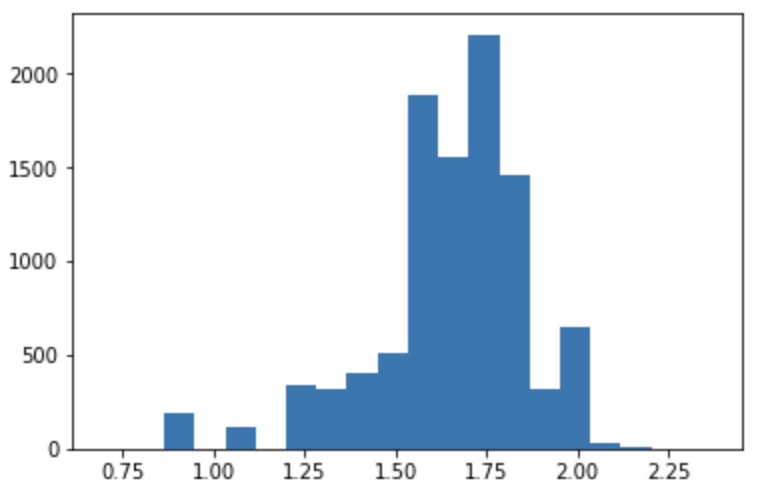
\includegraphics[scale=0.75]{PS2P3C.png}
\end{center}

\problempart % Problem 3d

See Jupyter Notebook for detailed results.

The bias of our estimate is,
$$ \mathrm{bias}(\hat{M}) = \boxed{0} $$
The standard error is,
$$ s_{\bar{X}} = \boxed{0.209} $$

\problempart % Problem 3e

See Jupyter Notebook for detailed results.

The confidence interval is,
$$ \boxed{\left(1.378, 2.319\right)} $$

\end{problemparts}

\newpage
\problem  % Problem 4

\begin{problemparts}

\problempart % Problem 4a

Our estimator is defined as,
$$ \hat{A}_a = \frac{K^2}{n^2} $$
Taking the expectation of the estimator,
\begin{align*}
    \mathbb{E}[\hat{A}_a] &= \mathbb{E}\left[\frac{K^2}{n^2}\right] \\
    &= \frac{\mathbb{E}[K^2]}{n^2}
\end{align*}
Since $K$ is a binomial random variable, we know the following,
$$ \mathbb{E}[K] = np,\quad \mathrm{var}(K) = np(1 - p) $$
From the definition of variance,
\begin{align*}
    \mathbb{E}[K^2] &= \mathrm{var}(K) + \mathbb{E}[K]^2 \\
    &= np(1 - p) + n^2 p^2
\end{align*}
Substituting this into our equation above,
\begin{align*}
    \mathbb{E}[\hat{A}_a] &= \frac{np(1 - p) + n^2 p^2}{n^2} \\
    &= \boxed{\frac{p(1 - p)}{n} + p^2}
\end{align*}
Using this, we can calculate the bias of the estimator,
\begin{align*}
    \mathrm{bias}(\hat{A}_a) &= \mathrm{E}[\hat{A}_a] - p^2 \\
    &= \frac{p(1 - p)}{n} + p^2 - p^2 \\
    &= \boxed{\frac{p(1 - p)}{n}}
\end{align*}

\problempart % Problem 4b

Our new estimator is defined as,
$$ \hat{A}_b = \frac{K^2}{n^2} - \frac{K (n - K)}{n^3} $$
Calculating the expectation (and immediately substituting the result
from Part A),
\begin{align*}
    \mathbb{E}[\hat{A}_b] &= \frac{p(1 - p)}{n} + p^2 - \mathbb{E}\left[\frac{K 
    (n - K)}{n^3}\right] \\
    &= \frac{p(1 - p)}{n} + p^2 - \frac{\mathbb{E}[K (n - K)]}{n^3} \\
    &= \frac{p(1 - p)}{n} + p^2 - \frac{n\mathbb{E}[K] - \mathbb{E}[K^2]}{n^3} \\
    &= \frac{p(1 - p)}{n} + p^2 - \frac{n^2 p - np(1 - p) - n^2 p^2}{n^3} \\
    &= \frac{p(1 - p)}{n} + p^2 - \frac{p}{n} +\frac{p(1 - p)}{n^2} + \frac{p^2}{n} \\
    &= \frac{np(1 - p) + n^2 p^2 - np + p(1 - p) + np^2}{n^2} \\
    &= \boxed{\frac{p(n^2 p - p + 1)}{n^2}}
\end{align*}
Using this, we can calculate the bias of the estimator,
\begin{align*}
    \mathrm{bias}(\hat{A}_b) &= \frac{p(n^2 p - p + 1)}{n^2} - p^2 \\
    &= \boxed{\frac{p (1 - p)}{n^2}}
\end{align*}
%%%%%%%%%%%%%%%%%%%%%%%%%%%%%%%%%%%%%%%%%%%%%%%%%%%%%%%%%%%%%%%%%%%%%%%%%%%%%%%%
This is smaller than the previous bias because, for all $n > 1$, $1 / n^2$ is 
less than $1 / n$.

\problempart % Problem 4c

Let our new, unbiased estimator be,
$$ \hat{A}_c = \frac{2\left(X_1 X_2 + X_3 X_4 + \ldots + X_{n - 1} X_n\right)}
{n} $$
We can show this is unbiased by taking the expectation,
\begin{align*}
    \mathbb{E}[\hat{A}_c] &= \mathbb{E}\left[\frac{2\left(X_1 X_2 + X_3 X_4 + 
    \ldots + X_{n - 1} X_n\right)}{n}\right] \\
    &= \frac{2 \mathbb{E}[X_1 X_2 + X_3 X_4 + \ldots + X_{n - 1} X_n]}{n} \\
    &= \frac{2 \left(\mathbb{E}[X_1 X_2] + \mathbb{E}[X_3 X_4] + \ldots + 
    \mathbb{E}[X_{n - 1} X_n]\right)}{n} \\
    &= \frac{2 \left(p^2 + p^2 + \ldots + p^2\right)}{n} \\
    &= \frac{2 n p^2}{2n} \\
    &= \boxed{p^2}
\end{align*}
Since the expectation is $p^2$, this estimator is unbiased.

We can also calculate the variance of our estimator,
\begin{align*}
    \mathrm{var}(\hat{A}_c) &= \mathrm{var}\left(\frac{2\left(X_1 X_2 + X_3 
    X_4 + \ldots + X_{n - 1} X_n\right)}{n}\right) \\
    &= \frac{4 \mathrm{var}\left(X_1 X_2 + X_3 X_4 + \ldots + X_{n - 1} 
    X_n\right)}{n^2} \\
    &= \frac{4 \left(\mathrm{var}(X_1 X_2) + \mathrm{var}(X_3 X_4) + \ldots 
    + \mathrm{var}(X_{n - 1} X_n)\right)}{n^2} \\
\end{align*}
We can compute the individual variances using the definition,
\begin{align*}
    \mathrm{var}(X_i X_j) &= \mathbb{E}[(X_i X_j)^2] - \mathbb{E}[X_i X_j]^2 \\
    &= \mathbb{E}[X_i^2 X_j^2] - \left(\mathbb{E}[X_i] \mathbb{E}[X_j]\right)^2 \\
    &= \mathbb{E}[X_i^2] \mathbb{E}[X_j^2] - p^4 \\
    &= \left(\mathrm{var}(X_i) + \mathbb{E}[X_i]^2\right) \left(\mathrm{var}(X_j) 
    + \mathbb{E}[X_j]^2\right) - p^4 \\
    &= \left(p(1 - p) + p^2\right) \left(p(1 - p) + p^2\right) - p^4 \\
    &= \left(p(1 - p) + p^2\right)^2 - p^4 \\
    &= p^2 - p^4
\end{align*}
Substituting this into the original equation,
\begin{align*}
    \mathrm{var}(\hat{A}_c) &= \frac{4 \left(p^2 - p^4 + \ldots + p^2 - p^4\right)}{n^2} \\
    &= \frac{4n\left(p^2 - p^4\right)}{2 n^2} \\
    &= \boxed{\frac{2 \left(p^2 - p^4\right)}{n}}
\end{align*}

\problempart % Problem 4d

Our new estimator is of the form,
$$ \hat{A}_d = \frac{K_1}{n / 2} \cdot \frac{K_2}{n / 2} $$
We can take the expectation of this estimator,
\begin{align*}
    \mathbb{E}[\hat{A}_d] &= \mathbb{E}\left[\frac{K_1}{n / 2} \cdot \frac{K_2}{n / 2}
    \right] \\
    &= \frac{4 \mathbb{E}[K_1 K_2]}{n^2} \\
    &= \frac{4 \mathbb{E}[\left(X_1 + \ldots + X_{n / 2}\right) \left(X_{n / 2 + 1} + 
    \ldots + X_n\right)]}{n^2} \\
    &= \frac{4 \mathbb{E}[X_1 X_{n / 2 + 1} + \ldots + X_{n / 2} X_n]}{n^2} \\
    &= \frac{4 \left(\mathbb{E}[X_1 X_{n / 2 + 1}] + \ldots + \mathbb{E}[X_{n / 2} 
    X_n]\right)}{n^2} \\
    &= \frac{4 \left( p^2 + \ldots + p^2 \right)}{n^2} \\
    &= \frac{4 n^2 p^2}{4 n^2} \\
    &= \boxed{p^2}
\end{align*}
Therefore, the estimator is unbiased.

\problempart % Problem 4e

The final estimator takes the form,
$$ \hat{A}_e = a + bK + c K^2 $$
We can take the expectation and substitute our findings from before,
\begin{align*}
    \mathbb{E}[\hat{A}_e] &= \mathbb{E}[a + bK + cK^2] \\
    &= a + b \mathbb{E}[K] + c \mathbb{E}[K^2] \\
    &= a + b n p + c \left(n (n - 1) p^2 + np\right) \\
    &= a + b n p + c n (n - 1) p^2 + cnp
\end{align*}
Since we want the $p^2$ by itself, we can set
$$ c = \frac{1}{n(n - 1)} $$
Substituting this in yields,
$$ \mathbb{E}[\hat{A}_e] =  a + b n p + p^2 + \frac{p}{n - 1} $$
Now we need to cancel the $p / (n - 1)$, so we set
$$ b = \frac{-1}{n(n - 1)} $$
Substituting this yields,
$$ \mathbb{E}[\hat{A}_e] =  a + p^2 $$
And we don't need $a$. The final unbiased estimator is,
$$ \hat{A}_e = \boxed{-\frac{K}{n(n - 1)} + \frac{K^2}{n(n - 1)}} $$

\end{problemparts}

\end{problems}

\end{document}


